\begin{figure}[h]
    \centering
    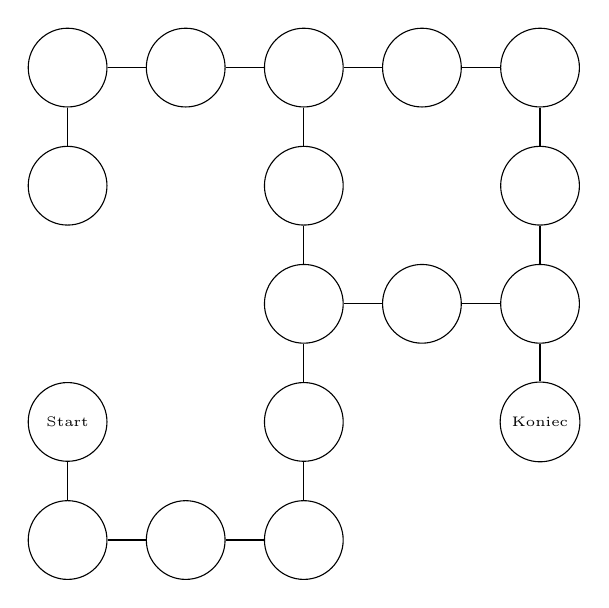
\begin{tikzpicture}[scale=1, every node/.style={circle,draw,minimum size=10mm}]
        \node (n00) at (0,0) {};
        \node (n01) at (0,1.5) {\tiny Start};
        \node (n03) at (0,4.5) {};
        \node (n04) at (0,6) {};

        \node (n10) at (1.5,0) {};
        \node (n14) at (1.5,6) {};

        \node (n20) at (3,0) {};
        \node (n21) at (3,1.5) {};
        \node (n22) at (3,3) {};
        \node (n23) at (3,4.5) {};
        \node (n24) at (3,6) {};

        \node (n32) at (4.5,3) {};
        \node (n34) at (4.5,6) {};

        \node (n41) at (6,1.5) {\tiny Koniec};
        \node (n42) at (6,3) {};
        \node (n43) at (6,4.5) {};
        \node (n44) at (6,6) {};

        \draw (n00) -- (n01);
        \draw (n03) -- (n04);
        \draw (n04) -- (n14);
        \draw (n00) -- (n10);
        \draw (n10) -- (n20);
        \draw (n20) -- (n21);
        \draw (n21) -- (n22);
        \draw (n22) -- (n23);
        \draw (n23) -- (n24);
        \draw (n14) -- (n24);
        \draw (n24) -- (n34);
        \draw (n41) -- (n42);
        \draw (n42) -- (n43);
        \draw (n43) -- (n44);
        \draw (n22) -- (n32);
        \draw (n32) -- (n42);
        \draw (n34) -- (n44);
    \end{tikzpicture}
    \caption{Graf reprezentujący labirynt z Rysunku \ref{fig:example_maze}.}
    \label{fig:maze_graph}
\end{figure}